\subsection{Common neural network blocks}
\label{appendix:blocks}



\subsection*{Multi-layer perception (MLP)}

Multi-layer perception (MLP) is a basic feed forward neural network architecture in which the input is passed through multiple layers of linear transformations (fully connected layers) and non-linear activation functions.

In short, we can think of MLP as a simple fully connected layers (sometimes called 'dense layer').








\subsection*{ResBlock}

\begin{figure}
    \centering
    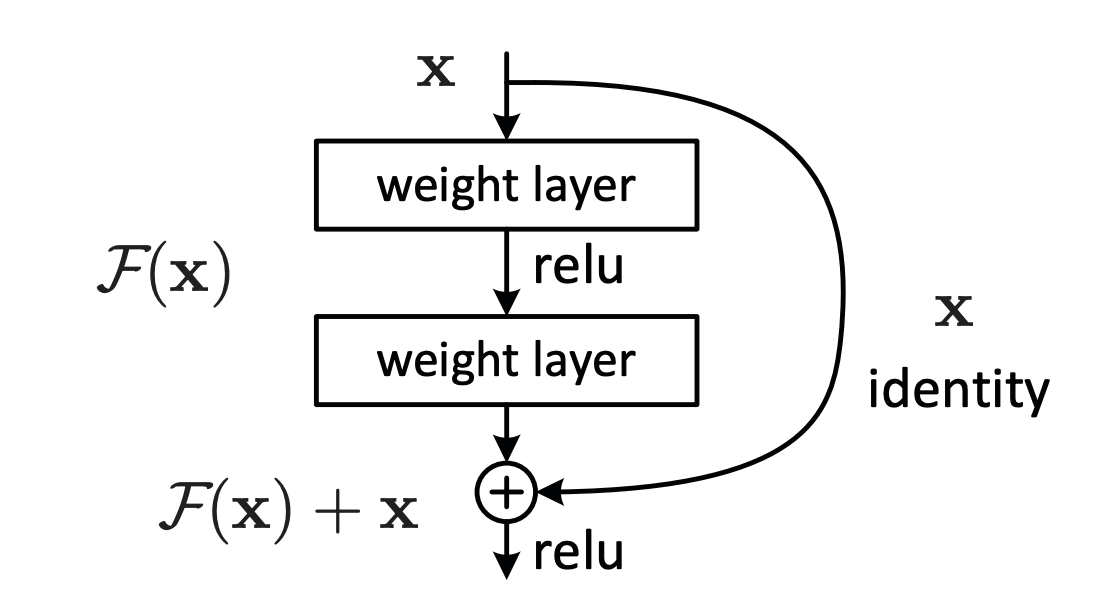
\includegraphics[width=0.4\textwidth]{images/appendix/blocks/resnet.png}
    \caption{\texttt{ResBlock} architecture, from the ResNet paper \cite{resnet}.}
    \label{fig:appendix_blocks_residual_block}
\end{figure}

Residual blocks (\texttt{ResBlock}) are skip-connection blocks that were introduced in the ResNet (Residual Network) paper \cite{resnet}. They are used to mitigate the exploding/vanishing gradient problem in very deep neural networks. A residual block allows the network to skip layers by adding identity shortcut connection (the input is added directly to the output of a few stacked layers). The main idea is that instead of learning the full mappings from input to output, the residual block only needs to learn a residual mapping (the difference between the input and output). Mathematically, residual mappings can be written as:

\begin{equation*}
    y = \mathcal{F} (x) + x
\end{equation*}

where $x$ is the input to the block, $\mathcal{F}$ is the residual function, and $y$ is the output of the block.

If a layer doesn't need to transform the input, the skip connection allows the network to learn an identity mapping, making it easier to optimize the model. Easier flow of gradients also mitigate the problem of vanishing/exploding gradients, where the gradients become too small or too large as they are backpropagated through the network, which is especially prominent in very deep networks.







\subsubsection{Normalization layers}
\label{appendix:blocks_norm}

\begin{figure*}
    \centering
    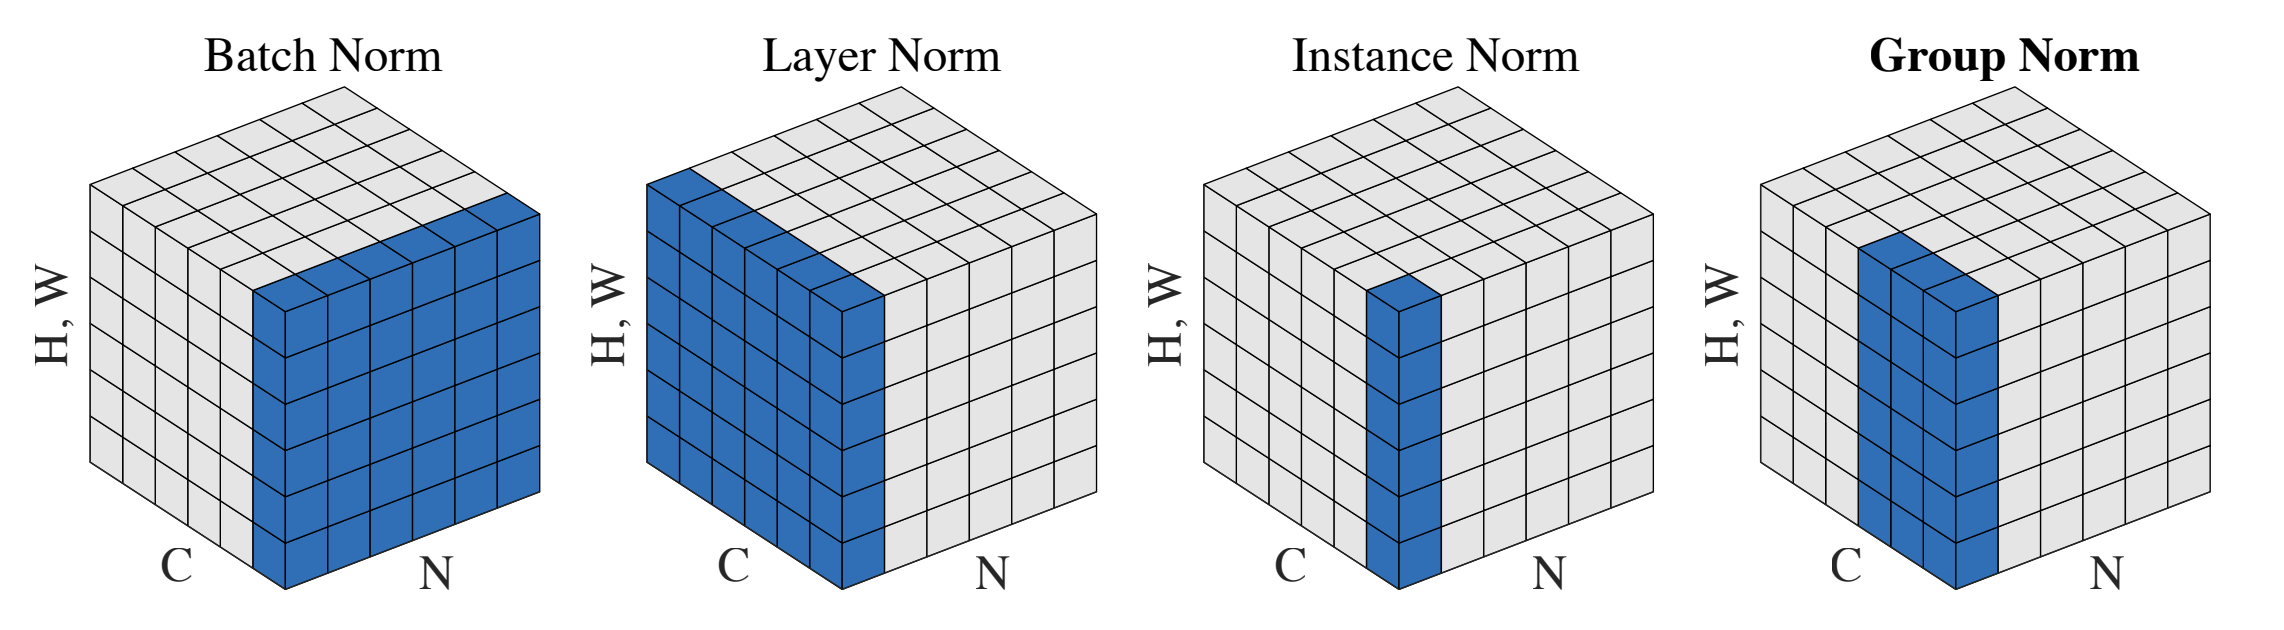
\includegraphics[width=0.75\textwidth]{images/appendix/blocks/norm.png}
    \caption{Visual comparison on mode of operations of \texttt{BatchNorm}, \texttt{LayerNorm}, \texttt{InstanceNorm}, and \texttt{GroupNorm} \cite{wu2018group}.}
    \label{fig:appendix_blocks_norm}
\end{figure*}

These layers ensure that the data is normalized in a way that the model can learn better. 

For example, we can think that the optimization problem is on a distribution that looks like very long ellipse, it would be hard for the model to reach minima. But if we normalize the data such that the distribution will fit a circle, then the optimization process will be easier. Normalization layers are used to change the shape of the distribution, scale it, and shift it to make the optimization process easier.

We use mean $\mu$ and variance $\sigma$ in the normalization layers:

\[ \mu = \frac{1}{H} \sum_{i=1}^{H} x_i \]

\[ \sigma = \sqrt{\frac{1}{H} \sum_{i=1}^{H} (x_i - \mu)^2} \]

where $H$ is the number of elements in the input $x$.






\subsection*{LayerNorm}

\texttt{LayerNorm}, introduced in a 2016 paper \cite{layernorm}, is a normalization block that normalizes the input across the feature channels rather than across the batch (as in \texttt{BatchNorm} block). This layer scales and shifts the input distribution. See figure \ref{fig:appendix_blocks_norm} for a visual comparison. In addition, because \texttt{LayerNorm} doesn't rely on batch size, it can be applied even in batch size of 1.

It's formally defined as:

\begin{equation*}
    \text{LayerNorm}(x) = \frac{x - \mu}{\sqrt{\sigma^2 + \epsilon}} \cdot \gamma + \beta
\end{equation*}

where $\mu = \mathbb{E}(x)$ is the mean of the input, $\sigma = \text{Var} (x)$ is the variance of the input, $\epsilon$ is a small constant to avoid division by zero, and $\gamma, \beta$ are learnable parameters. The $\gamma$ and $\beta$ parameters scale and shift the normalized input.










\subsection*{BatchNorm}

\texttt{BatchNorm} was introduced in a 2015 paper \cite{batchnorm}\footnote{A great YouTube video explaining why batch normalization speeds up the training process (by not overshooting in the learning rate) is available at \href{https://www.youtube.com/watch?v=DtEq44FTPM4}{this link}.}.

Let $\mu_B$ be the mean of the mini-batch, and $\sigma^2_B$ be the variance of the mini-batch, and $m$ be the number of samples in the mini-batch. The operation of \texttt{BatchNorm} is defined as:

\begin{equation*}
    \text{BatchNorm}(x) = \frac{x - \mu_B}{\sqrt{\sigma^2_B + \epsilon}} \cdot \gamma + \beta
\end{equation*}

where $\gamma, \beta$ are learnable parameters, and $\epsilon$ is a small constant to avoid division by zero. The $\gamma$ and $\beta$ parameters scale and shift the normalized input.








\subsection*{GroupNorm}

\texttt{GroupNorm} was introduced in a 2018 paper \cite{wu2018group}. \texttt{GroupNorm} strikes a balance between \texttt{LayerNorm} and \texttt{BatchNorm}, where it normalizes the input across the feature channel but not all of it, rather it normalizes groups of input features, hence the name.

The operation of \texttt{GroupNorm} is defined as:

\begin{equation*}
    \text{GroupNorm}(x) = \frac{x - \mu}{\sqrt{\sigma^2 + \epsilon}} \cdot \gamma + \beta
\end{equation*}

where $\mu = \mathbb{E}(x)$ is the mean of the input, $\sigma = \text{Var} (x)$ is the variance of the input, $\epsilon$ is a small constant to avoid division by zero, and $\gamma, \beta$ are learnable parameters. The $\gamma$ and $\beta$ parameters scale and shift the normalized input.




% \subsection*{Adaptive Layer Normalization (adaLN)}

% % TODO: Complete
% Adaptive Layer Normalization (adaLN) blocks are ...






\subsection{3D Convolutions}
\label{appendix:blocks_3dconv}

\begin{figure}
    \centering
    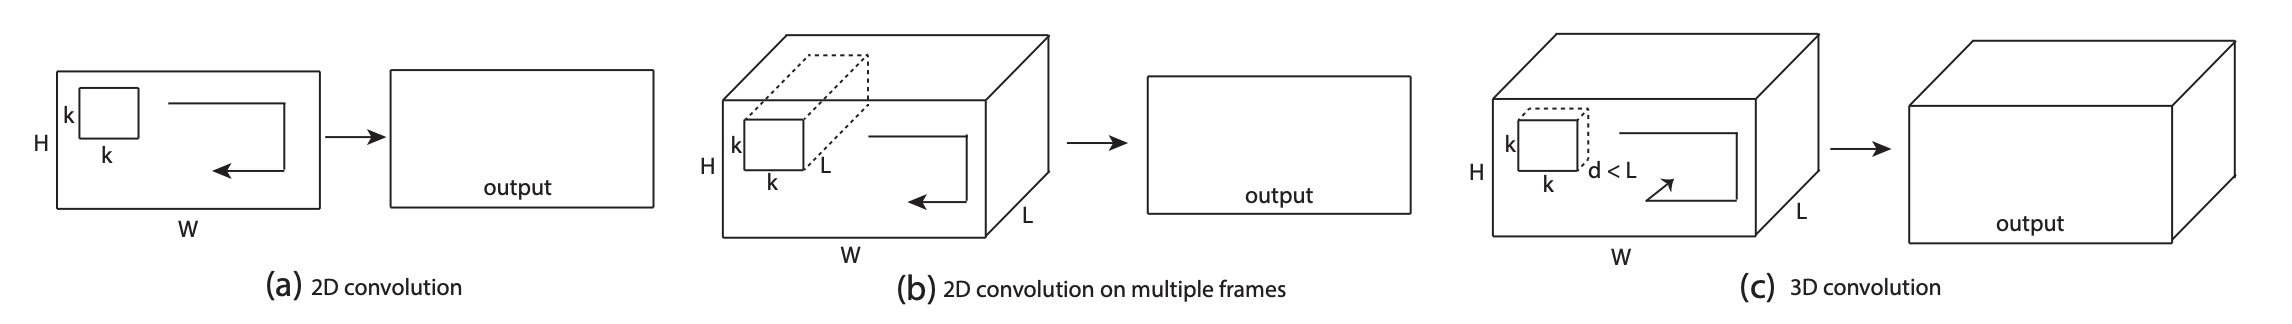
\includegraphics[width=1\textwidth]{images/appendix/blocks/3d_conv.png}
    \caption{2D and 3D convolution operations. (a) Applying 2D convolution on image results in an image (2D tensor). (b) Applying 2D convolution on video (multiple frames) also results in an 2D vector. (c) Applying 3D convolution on video results in a 3D tensor with a temporal dimension. Figure from a 2014 paper \cite{tran2015learning}.}
    \label{fig:appendix_blocks_3dconv}
\end{figure}

Figure \ref{fig:appendix_blocks_3dconv} illustrates 2D and 3D convolutions.

3D convolution extends 2D convolution by adding a depth dimension, useful for temporal data like videos. The kernel moves through all three dimensions: width, height, and depth (often known as the temporal dimension for video, across frames).

Given an input of size $H \times W \times D$ and a kernel of size $k_h \times k_w \times k_d$, the 3D convolution operation is defined as:

\begin{equation*}
    y_{i,j,k} = \sum_{l=0}^{k_d} \sum_{m=0}^{k_h} \sum_{n=0}^{k_w} x_{i+m,j+n,k+l} \cdot w_{m,n,l}
\end{equation*}

Like 2D convolution, 3D convolution can use stride, padding, and dilation. Stride refers to the kernel's movement steps, padding adds zeros to the input to preserve output size, and dilation controls the spacing between kernel elements.

For both 2D and 3D convolutions, the number of input and output channels determines the number of filters applied.
